% vim: set spell : spelllang=en_gb
\title{\bf Dynamic priority broadcasting channels:\\
	a multi-objective planning problem}
\author{Chiel Kooijman - 5743028\\University of Amsterdam}
\documentclass{article}
\usepackage{graphicx,amsmath}
\usepackage[round]{natbib}
\usepackage{multicol}
\usepackage{caption}
\usepackage{subcaption}
\usepackage{geometry}
\def\keywords{\vspace{.5em}
	{\textbf{Keywords}:\,\relax
}}
\def\endkeywords{\par}
\newenvironment{tablehere}
{\def\@captype{table}}
{}

\newenvironment{figurehere}
{\def\@captype{figure}}
{}

\date{}
\setlength{\textwidth}{6.5in}
\setlength{\oddsidemargin}{0in}
\setlength{\evensidemargin}{0in}
\thispagestyle{empty}
\begin{document}
	\maketitle
	\begin{keywords}
		Dynamic Programming, MDP, Markov Decision Process, Multiobjective,
		Planning, Broadcasting Channel, Dynamic Priority
	\end{keywords}


	\begin{multicols}{2}

	\section{Introduction}
	\label{sec:introduction}
	In this research we extend the broadcasting channel problem as defined by
	\citet{ooi1996decentralized}, in order to account for situations in which
	multiple objectives are important, such as workload distribution in a data
	environment, distribution of traffic, or prioritisation of more important
	messages, in addition to throughput.
	In section \ref{sec:problem_definition} we redefine the problem to account
	for these considerations. Section \ref{sec:approach} covers the methods used
	to meet these requirements.
	% section introduction (end)

	\section{Problem definition}
	\label{sec:problem_definition}
	Multiple agents broadcast messages over a single channel, but only one
	message can be sent at any time, otherwise conflicts will arise and no
	message will come through. After a message is sent, the agents will know
	whether a message was sent, a conflict has arisen, or no message was sent.
	Agents have a single buffer that may contain a message. An example of a
	two-agent setup is shown in figure \ref{fig:agents_ee}.

	\begin{figurehere}
		\centering
		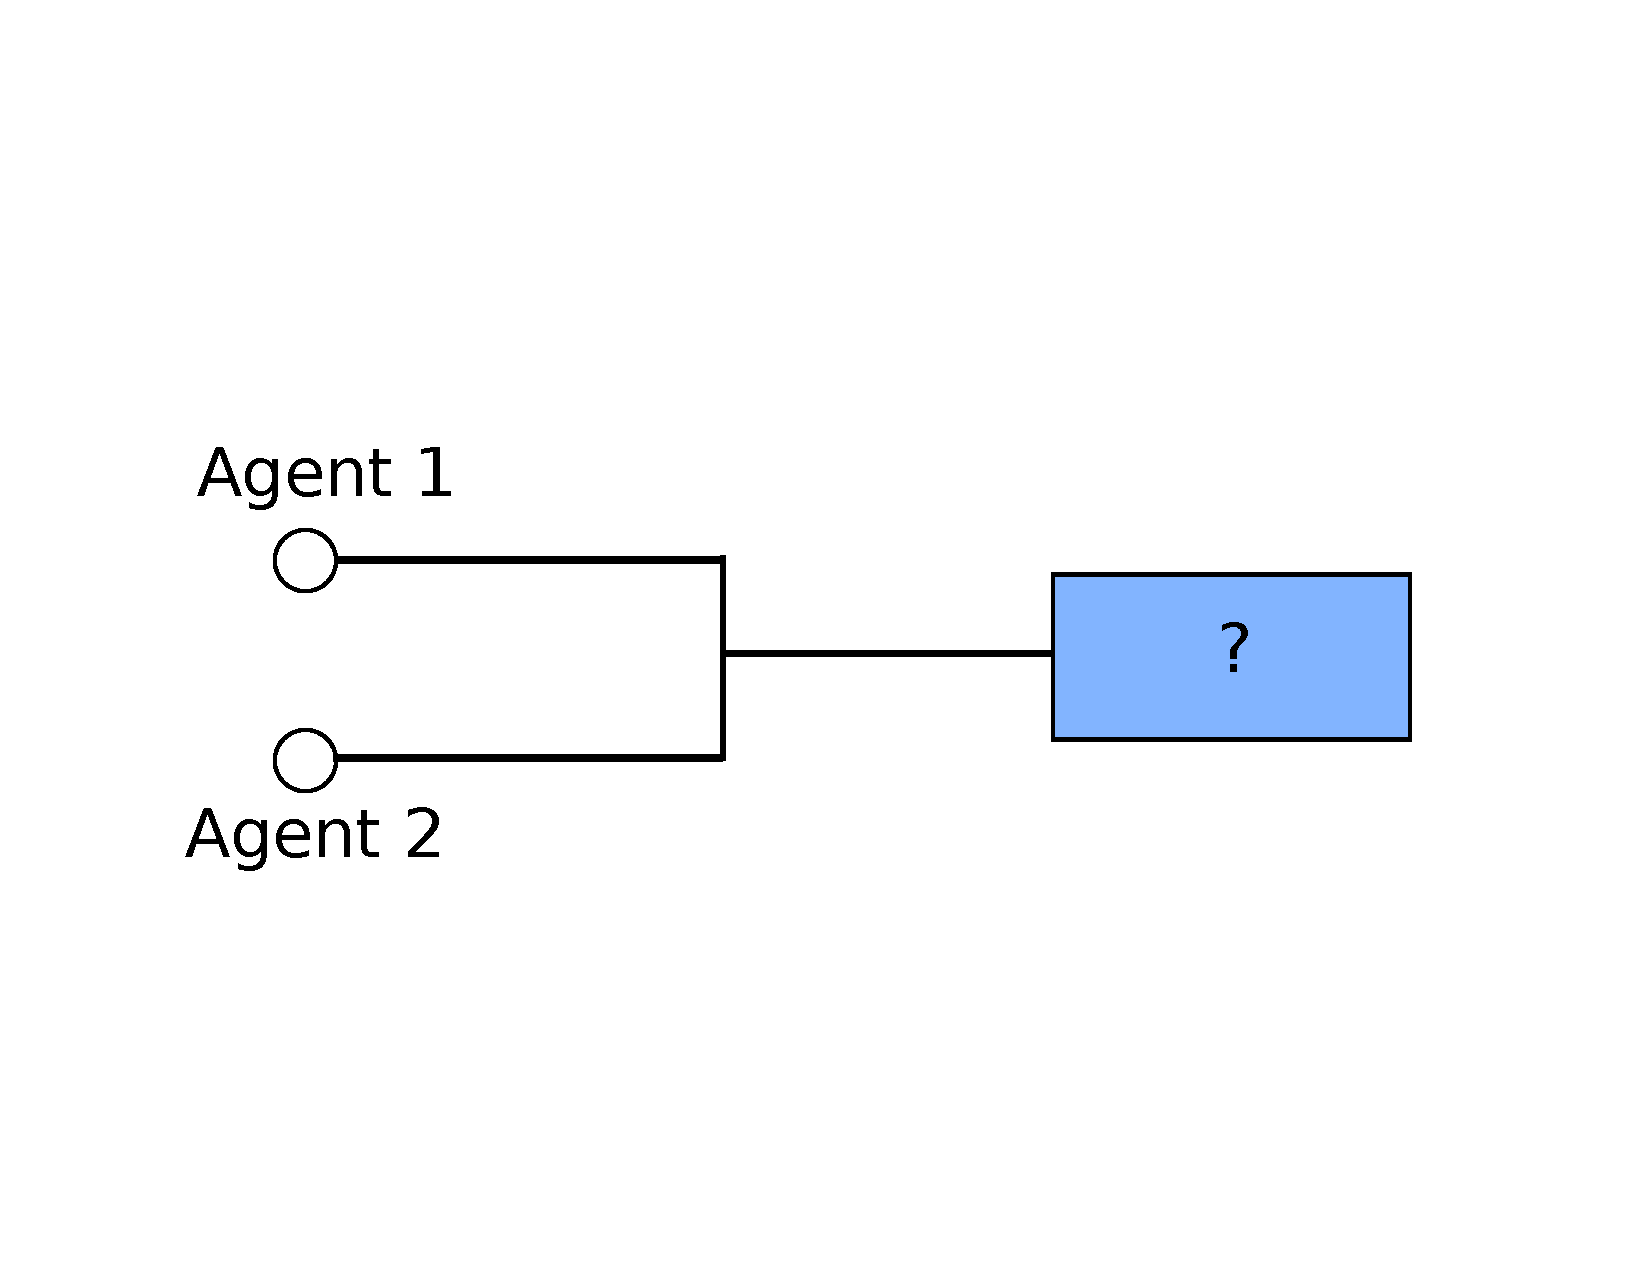
\includegraphics[scale=0.3]{images/agents_ee}
		\captionof{figure}{A setup with two agents}
	   \label{fig:agents_ee}
	\end{figurehere}

	At any concrete time-step an agent $i$ with an empty buffer may get a new
	message with probability $p_i(s' |s, \vec{a})$ in a fully observable Markov
	decision process (MDP), and $p_i(s' \vec{o}|s, \vec{a})$ in a partially
	observable Markov decision process (POMDP) \citep{hansen2004dynamic}.

	The problem of optimising throughput has been solved for POMDPs
	\citep{ooi1996decentralized, hansen2004dynamic}, but in this case we would
	also like to avoid dominance of a single agent over the channel.

	Finding an optimal policy in terms of both throughput and dominance will
	first be solved for a fully observable MDP with two agents. Then the aim is
	to generalise towards any number of agents, a POMDP, and/or \emph{learning}
	the policy, dependent on the amount of time available.

	\citet{hansen2004dynamic} have provided a solution with dynamic programming.
	This method will be extended so that for any weight vector $\vec{w}$ it will
	return the optimal Pareto-optimal set of solutions $\vec{w} \cdot
	\vec{V}^\pi$ \citep{vamplew2011empirical}, in a reward representation that
	can dynamically adapt priorities by changing the weights
	\citep{barrett2008learning,natarajan2005dynamic}.

	This research will evaluate the computational complexity of different
	approaches, while working towards a more realistic setup. It aims to
	combine dynamic priority with features such as predicting the transitional
	probabilities, which are presumably not very random in real-world
	situations. Other possibilities are partial observability, where agents are
	unaware of each others states, or working without an event horizon, so that
	it may work on any time-frame.

	If this problem is solved efficiently this may improve efficiency of network
	communications, because less time is spent on communicating about data, and
	buffer sizes can be decreased in modems where multiple devices are connected
	through this modem.
	% section problem_definition (end)

	\section{Approach}
	\label{sec:approach}

		\subsection{Reward Representation}
		\label{sub:reward_representation}
		There are several ways to represent throughput and dominance in a vector.
		One approach is to have a two-dimensional vector $\vec{r}$ that contains
		the total throughput and some measure of dominance, for instance entropy
		or variance. An advantage of this approach is that the size of the reward
		vector is independent of the number of agents.

		Another way is to represent the vector as an $n$-dimensional vector:
		$$\vec{r} = \begin{bmatrix}
			t_1\\
			\vdots\\
			t_n\\
		\end{bmatrix}$$
		where $n$ is the number of agents, and each value represents the
		throughput of the corresponding agent. An advantage is that the vector
		contains more information than in the aforementioned representation,
		which allows us to use different measures of optimality, but
		there are many more states when the number of agents increases. It does
		however allow for prioritising messages, and when we choose not to
		prioritise, the number of states can be greatly reduced, because every
		vector is equal to all of its permutations (provided we reorder the state
		vector and the reward vector in the same way).
		For example in a two-agent system, a state with a reward vector $\vec{r}$
		and function parameter $\vec{\theta}$
		vectors
		$$ f_{\vec{\theta}}(\vec{r})~\textrm{with}~\vec{r} = \begin{bmatrix}
			7\\
			3\\
		\end{bmatrix},~
		\vec{\theta} = \begin{bmatrix}
			w_1\\
			w_2\\
		\end{bmatrix}$$
		the value is equal to that of
		$$ f_{\vec{\theta}}(\vec{r})~\textrm{with}~\vec{r} = \begin{bmatrix}
			3\\
			7\\
		\end{bmatrix},~
		\vec{\theta} = \begin{bmatrix}
			w_2\\
			w_1\\
		\end{bmatrix}$$
		because all agents are equal and connected to the network in the same
		way.

		For these reasons the second representation was chosen.
		% subsection reward_representation (end)

		\subsection{State Representation}
		\label{sub:state_representation}
		The Bellman equation \ref{eq:bellman} describes the value $V$ of a state
		$s$ given policy $\pi$. It is defined by return $R$ that is obtained in
		state $s$, plus the expected return in the following states $s'$given the
		policy. Discount value $\gamma$ is a value in $[0, 1)$, and defines the
		weight of future rewards. Low values can be seen as making the agent
		impatient, because a states value is mostly defined by expected return in
		the near future.
		\begin{equation}
		\displaystyle
		V(s)^\pi = R(s) + \gamma\sum_{s'} P(s'|s, \pi(s)) V^\pi(s')
		\label{eq:bellman}
		\end{equation}

		In a system with an event horizon we can represent a state as a vector of
		booleans, that represents for each agent whether it has a message to send
		or not. Furthermore, discounting is unnecessary when calculating state
		values, whereas in a system without a horizon discounting the reward is
		necessary to make the values converge. With Dynamic Programming (DP) we
		can calculate the optimal policy. Values for the states can be redefined
		as shown in equation \ref{eq:bellman_dp}.

		\begin{equation}
		\displaystyle
		V(s)^* = R(s) + \max_a \sum_{s'} P(s'|s, a) V^*(s')
		\label{eq:bellman_dp}
		\end{equation}

		In our case it may be more useful to represent values of state-action
		pairs, as the immediate return $R$ is dependent on the action given the
		state. Equation \ref{eq:bellman_q} shows how this value $Q$ can be
		calculated.
		\begin{equation}
		\displaystyle
		Q(s, a)^* = \sum_{s'} P(s'|s, a) \left(R(s, a) + \max_{a'} Q^*(s', a')\right)
		\label{eq:bellman_q}
		\end{equation}

		For each state only Pareto-optimal rewards need to be saved, because they
		contain all values for any definition of optimality.

		Equation \ref{eq:pareto} shows the definition for the Pareto-optimal set.
		\begin{equation}
			\label{eq:pareto}
			\Big\{ V\, \Big| \, \forall V'[ V \neq V' \land \exists n [V_n > V'_n]] \Big\}
		\end{equation}
		An example of a Pareto-optimal set for a two-dimensional system is shown in
		figure \ref{fig:pareto}.

	\begin{figurehere}
		\centering
		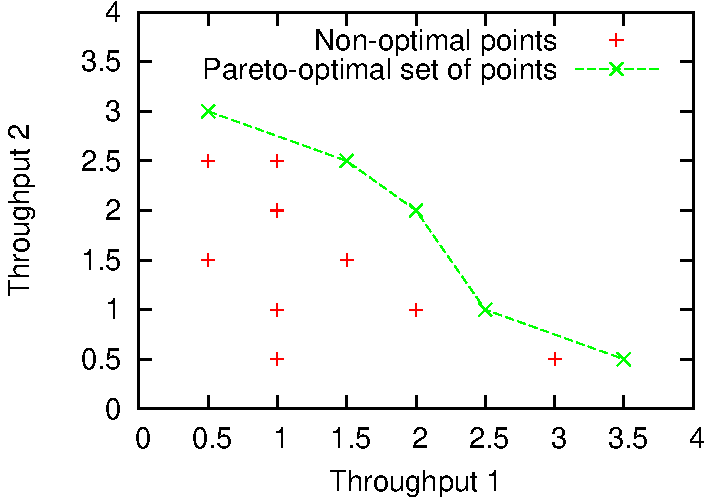
\includegraphics[scale=0.68]{images/pareto}
		\captionof{figure}{Pareto-optimal set in a two-dimensional system}
	   \label{fig:pareto}
	\end{figurehere}

		% subsection state_representation (end)

		\subsection{Comparisons}
		\label{sub:comparisons}
		For this research the algorithm can be compared to the turn-based
		implementation where each agent may only send a message in its own turn.
		% subsection comparisons (end)
	% section approach (end)

	\end{multicols}
	\section{Results}
	\label{sec:results}
	Table \ref{tab:turns} shows that the turn-based approach is more efficient
	as the number of agents and the probability of obtaining a new message
	increases. This is because after the all agents have had their first turn,
	the probability of having a message to send is $P(m)^n$, as there are
	$n$ times that a new message can fill the buffer with probability $P(m)$.

	\begin{table}[h]
		\centering
		\begin{tabular}{|r|rrrrr|}
			\hline
			& 1 agent & 2 agents & 3 agents& 4 agents& 5 agents\\
			\hline
			$p=0.1$ & 100157 & 190211 & 271604 & 344064 & 410397\\
			$p=0.2$ & 200015 & 360030 & 488788 & 590683 & 672028\\
			$p=0.5$ & 500050 & 749407 & 875208 & 937568 & 968696\\
			$p=0.7$ & 699996 & 909630 & 972937 & 991940 & 997638\\
			\hline
		\end{tabular}
		\caption{Total throughput for turn-based policy after 1000000 turns}
		\label{tab:turns}
	\end{table}

	\newgeometry{textwidth=\paperwidth,layouthoffset=.75cm}
	\begin{figure}
		\begin{subfigure}[b]{0.3\textwidth}
			\centering
			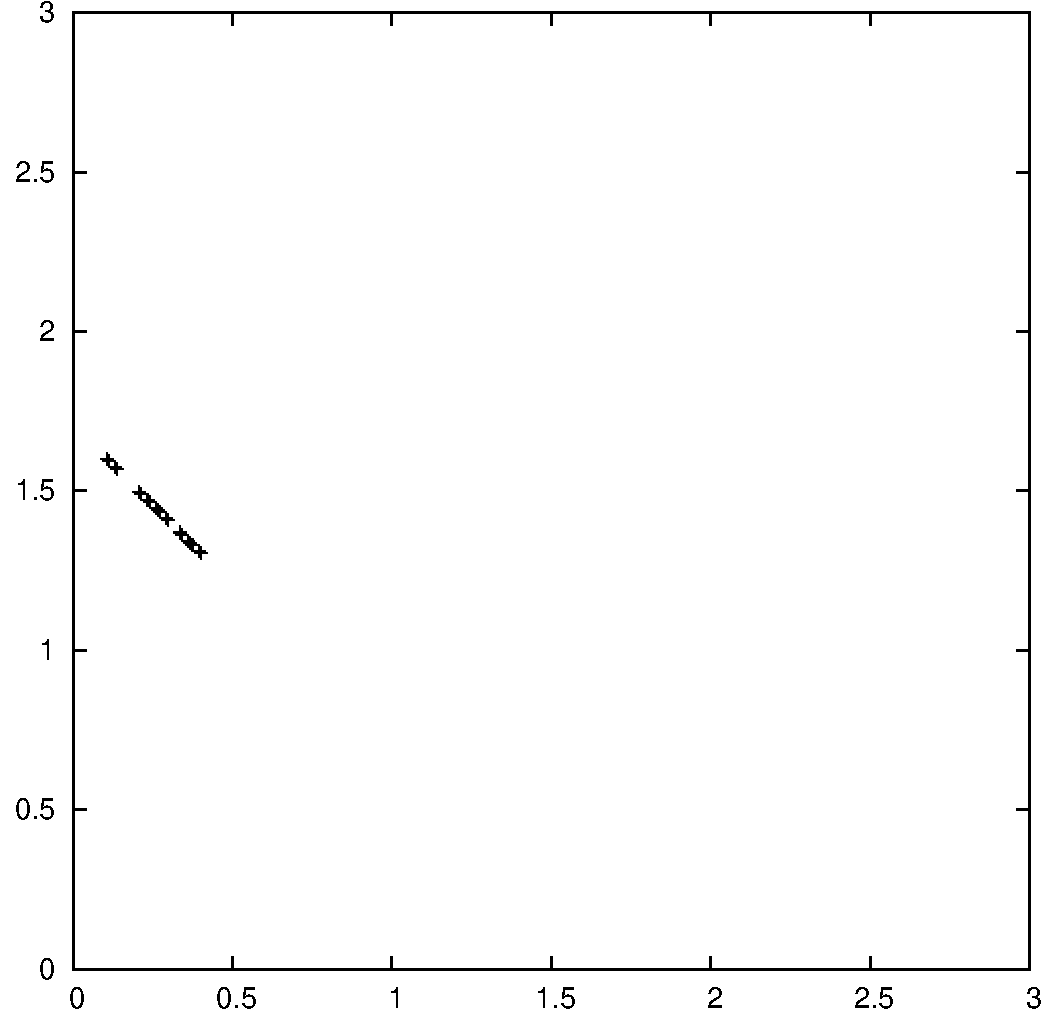
\includegraphics[width=\textwidth]{images/t2s0}
			\caption{s=(e,e)}
			\label{fig:t2s0}
		\end{subfigure}
		~
		\begin{subfigure}[b]{0.3\textwidth}
			\centering
			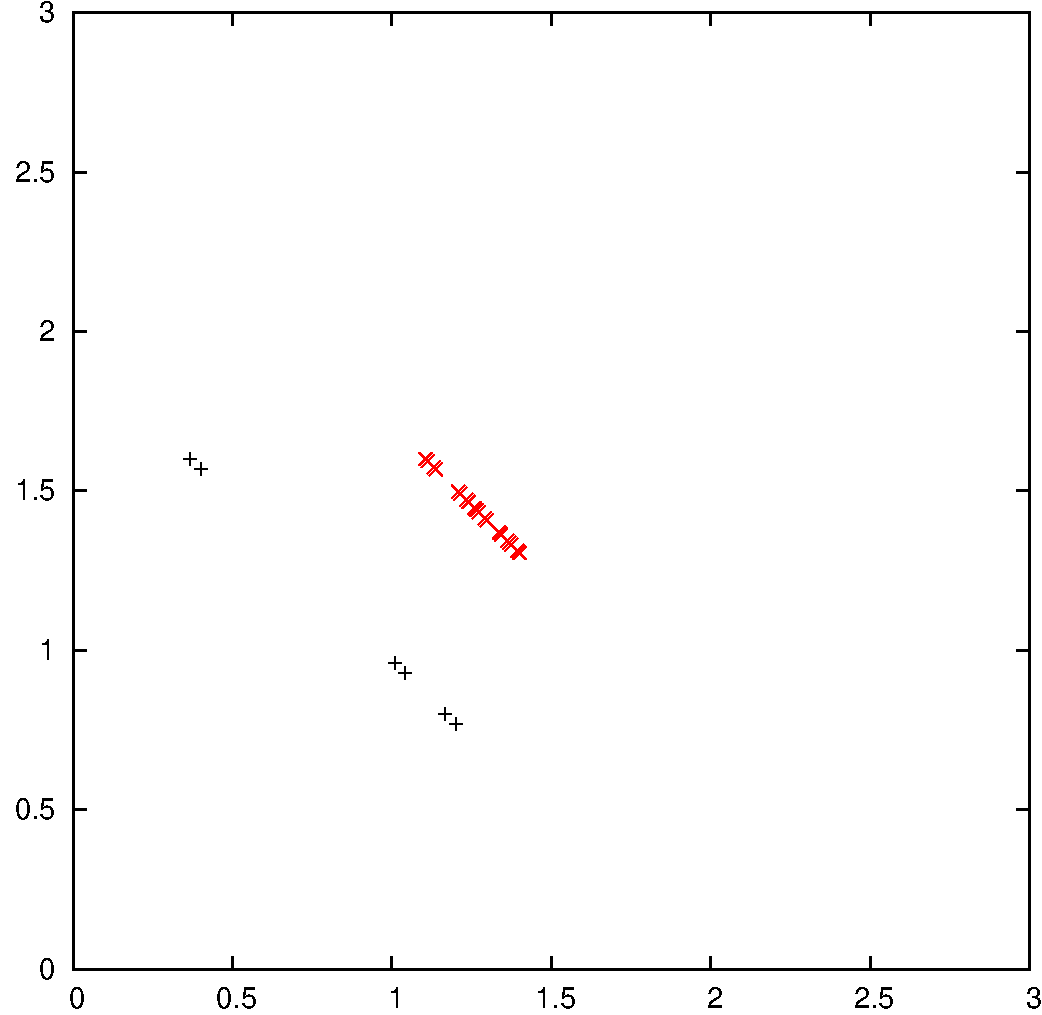
\includegraphics[width=\textwidth]{images/t2s1}
			\caption{s=(m,e)}
			\label{fig:t2s1}
		\end{subfigure}
		~
		\begin{subfigure}[b]{0.3\textwidth}
			\centering
			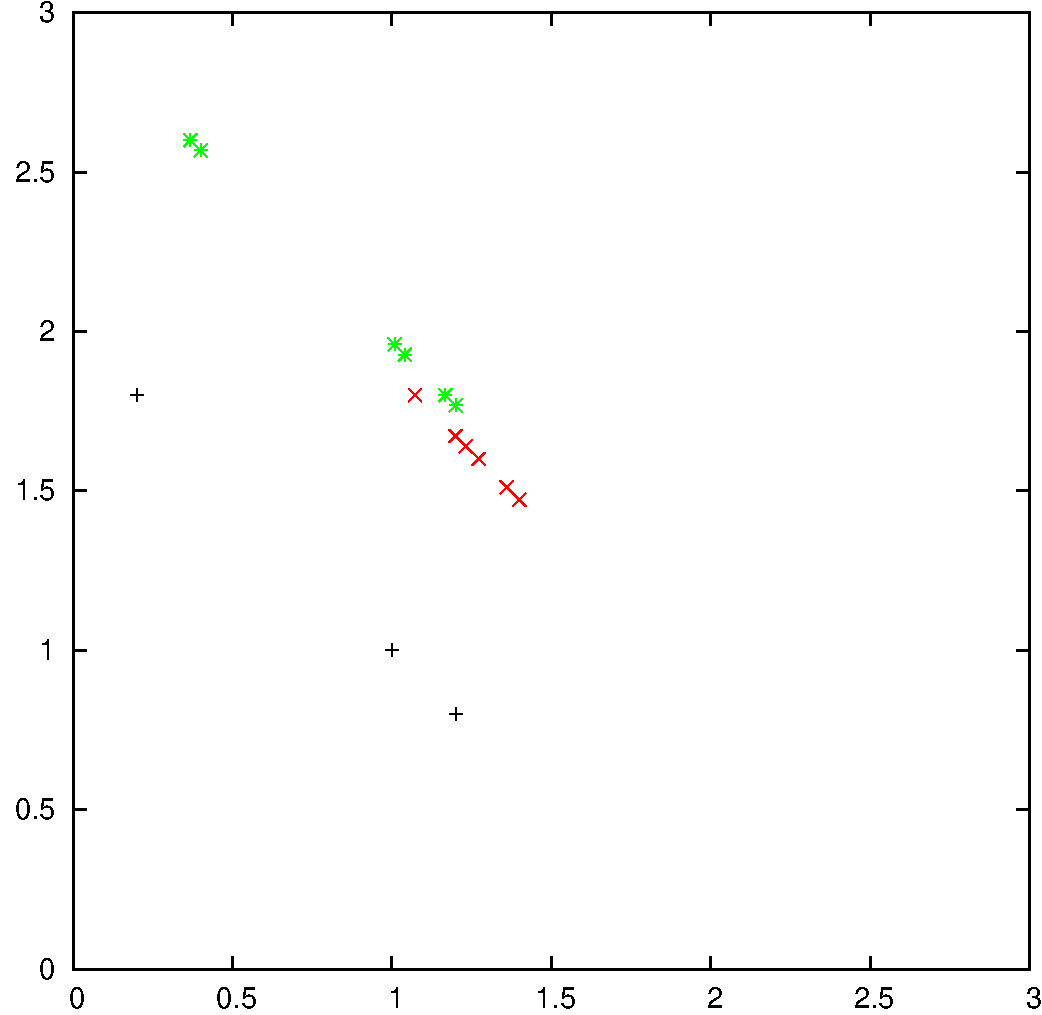
\includegraphics[width=\textwidth]{images/t2s3}
			\caption{s=(m,m)}
			\label{fig:t2s3}
		\end{subfigure}
		\caption{Time step 2}
	\end{figure}

	\begin{figure}
		\begin{subfigure}[b]{0.3\textwidth}
			\centering
			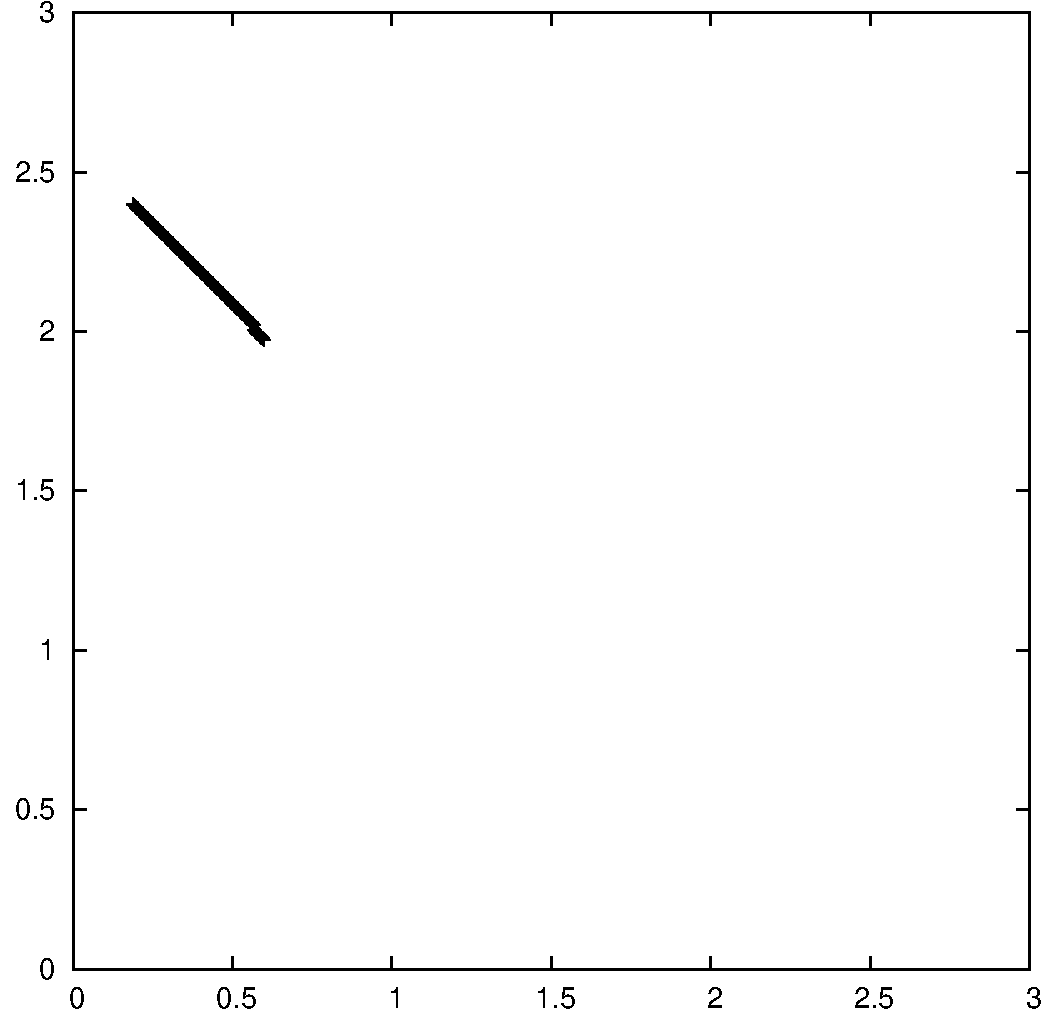
\includegraphics[width=\textwidth]{images/t3s0}
			\caption{s=(e,e)}
			\label{fig:t3s0}
		\end{subfigure}
		~
		\begin{subfigure}[b]{0.3\textwidth}
			\centering
			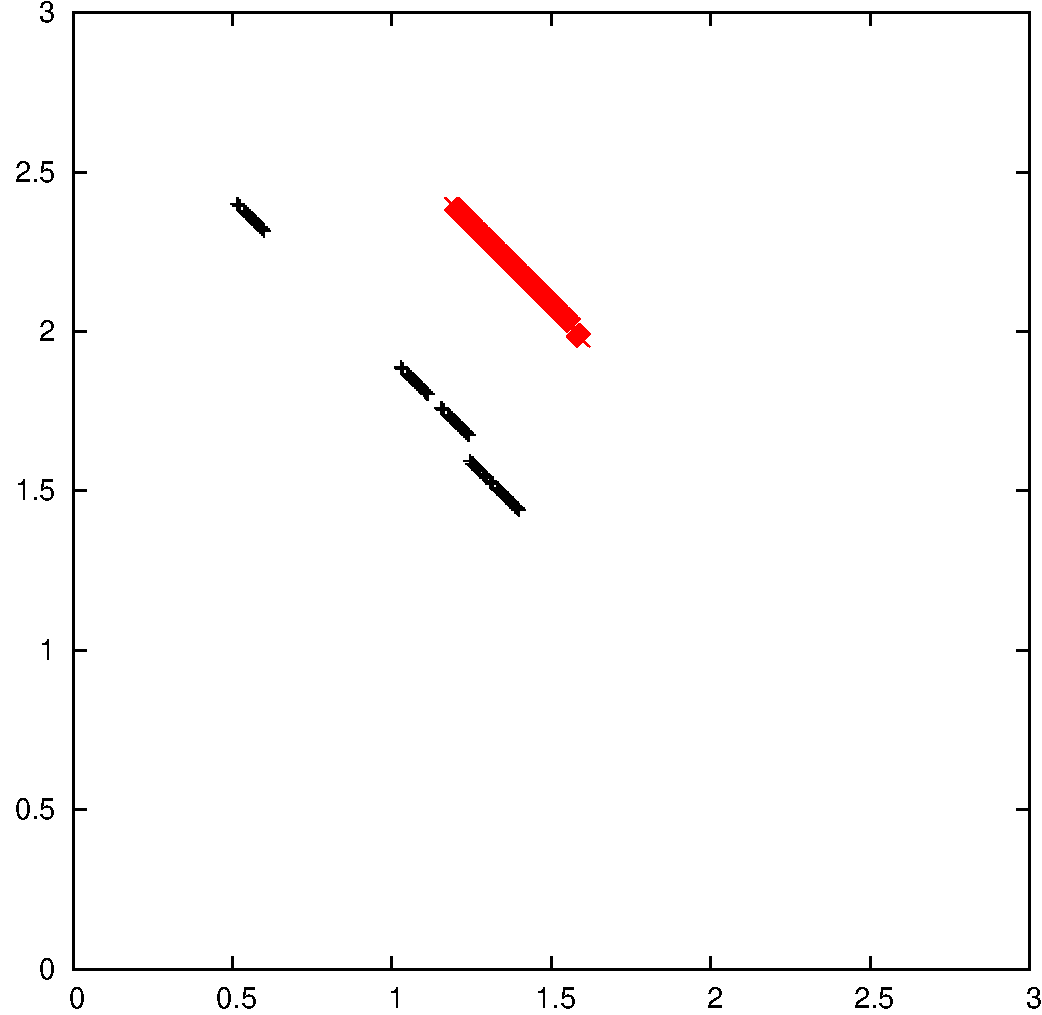
\includegraphics[width=\textwidth]{images/t3s1}
			\caption{s=(m,e)}
			\label{fig:t3s1}
		\end{subfigure}
		~
		\begin{subfigure}[b]{0.3\textwidth}
			\centering
			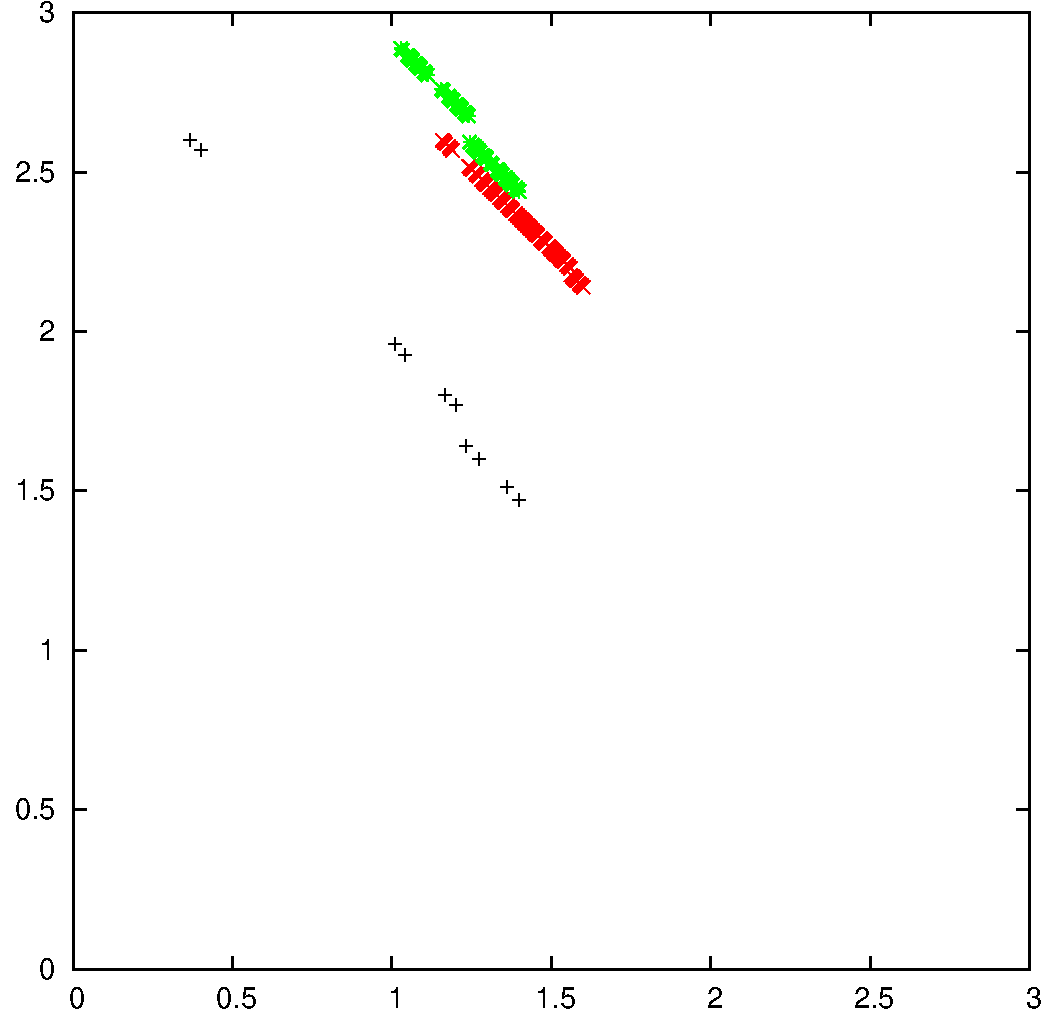
\includegraphics[width=\textwidth]{images/t3s3}
			\caption{s=(m,m)}
			\label{fig:t3s3}
		\end{subfigure}
		\caption{Time step 3}
	\end{figure}
	\restoregeometry
	% section results (end)
	\pagebreak

	\bibliographystyle{plainnat}
	\bibliography{references}
\end{document}

